\documentclass{beamer}
\usepackage{ngerman}
\usepackage[utf8]{inputenc}
\usepackage{pgf}
\usepackage{verbatim}
\usepackage{listings}
\usepackage[]{hyperref} 
\usepackage{multicol}
\beamertemplatenavigationsymbolsempty

\usetheme{Szeged}

\title{HadoopDB\\ ein großer Schritt in die falsche Richtung}
\subtitle[]{Seminar 01912\\ Sommersemester 2011}
\date{\today}
\author[T. Koch]{Thomas Koch}
\institute[Fernuni Hagen]{Lehrgebiet Datenbanksysteme für neue Anwendungen\\ Fernuniversität Hagen}

\begin{document}
  \begin{frame}
    \titlepage
  \end{frame}

  \begin{frame}
    \tableofcontents{}
  \end{frame}

\section{Ende einer Ära}
\begin{frame}{Zeiten ändern sich \ldots}
  \begin{itemize}
    \item Hardware: Speicher, Geschwindigkeit
    \item Kosten Mensch/Maschine
    \item Parallelität
    \item Anwendungsbereiche
  \end{itemize}
  aus: The End of an Architectural Era (It’s Time for a Complete Rewrite) von 
Stonebraker, Michael; Abadi, Daniel J. et al.
\end{frame}

\begin{frame}{MapReduce gegen parallele Datenbanken}
  MapReduce: A major step backwards (Stonebraker)
  \begin{itemize}
    \item MapReduce ist nicht neu (und nicht gleich Hadoop)
    \item keine Schemas
    \item keine höhere Abfragesprache
    \item fehlende Features: Import, sekundäre Indizes, Updates, Transaktionen, Integrität, Views
  \end{itemize}
\end{frame}

\section{Benchmarks}
\begin{frame}{}
  maximal 100 Server
  \begin{quote}
     ``Since few data sets in the world even approach a petabyte in size, it is not at all clear how many MR users really need 1.000 nodes.'' (Stonebraker)
  \end{quote}
  \begin{quote}<2>
     ``I think there is a world market for maybe five computers''
   
     ``640K ought to be enough for anybody''
  \end{quote}
\end{frame}

\begin{frame}{Kritik der Benchmarks}
  \begin{itemize}
    \item keine (echte) Fehlertoleranz
    \item Datenladephase
    \item Problemarten
  \end{itemize}
\end{frame}

\section{HadoopDB}

\begin{frame}{Anforderungen}
  \begin{itemize}
    \item Performanz
    \item Fehlertoleranz
    \item Heterogene Server
    \item Flexible / Erweiterbare Abfrageschnittstelle
  \end{itemize}
  (Energieeffizienz?)
\end{frame}

\begin{frame}{Architektur}
  \begin{center}
    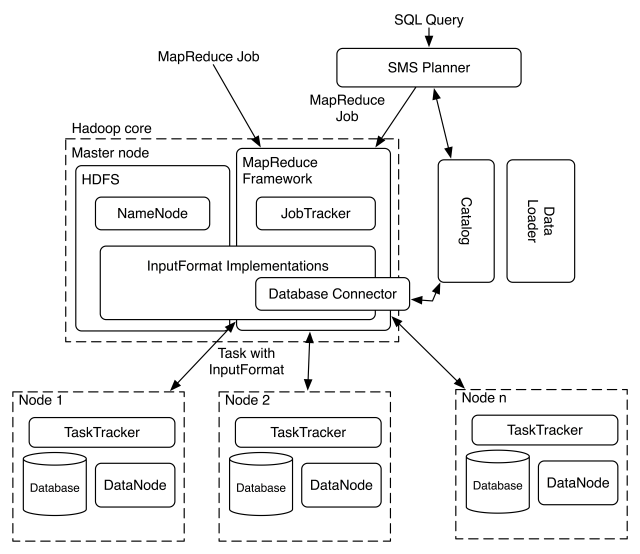
\includegraphics[width=0.7\textwidth]{../ausarbeitung/images/hadoopdb-arch.png}    
  \end{center}
\end{frame}

\begin{frame}{Datenladephase}
  \begin{enumerate}
    \item globaler Hasher (2r, 2w + 1 network copy)
    \item Export ins lokale Dateisystem (1r, 1w)
    \item lokaler Hasher (1r, 1w)
    \item Import in lokale Datenbank (1r, 1w + Indizes)
  \end{enumerate}
  \pause
  5x lesen, 5x schreiben
\end{frame}

\begin{frame}[fragile]{SQL-MapReduce-SQL Planer}
\begin{verbatim}
SELECT YEAR(saleDate), SUM(revenue)
FROM sales GROUP BY YEAR(saleDate)
\end{verbatim}
\end{frame}

\begin{frame}{SQL-MapReduce-SQL Planer}
  \begin{center}
    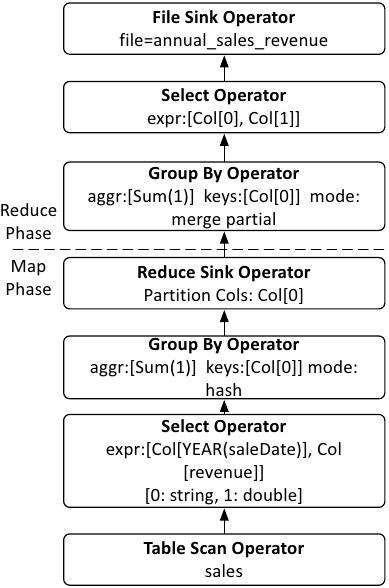
\includegraphics[height=0.8\textheight]{../ausarbeitung/images/hadoopdb-reduce-map-phase_a.png}    
  \end{center}
\end{frame}
\begin{frame}{SQL-MapReduce-SQL Planer}
  \begin{center}
    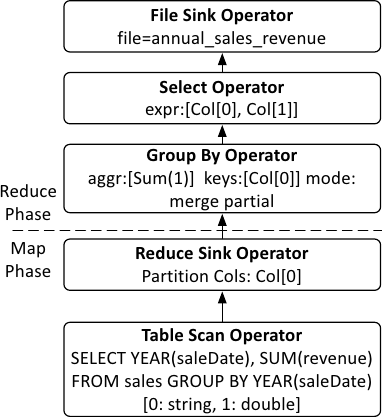
\includegraphics[height=0.8\textheight]{../ausarbeitung/images/hadoopdb-reduce-map-phase_c.png}    
  \end{center}
\end{frame}
\begin{frame}{SQL-MapReduce-SQL Planer}
falls per YEAR(saleDate) partitioniert wurde:
  \begin{center}
    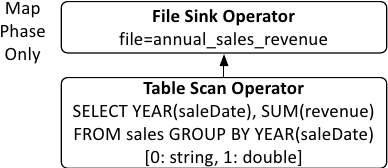
\includegraphics[height=0.3\textheight]{../ausarbeitung/images/hadoopdb-reduce-map-phase_b.png}    
  \end{center}
\end{frame}

\begin{frame}{weitere HadoopDB Komponenten}
  \begin{itemize}
  \item Datenbank Connectoren
  \item Catalog:
    \begin{itemize}
    \item Datenbankverbindungsparameter
    \item Metainformationen der Tabellen
    \item Speicherorte von Replikationen
    \item Partitionseigenschaften
    \end{itemize}
  \end{itemize}
\end{frame}

\begin{frame}[fragile]{Grep Task}
\begin{verbatim}
SELECT * FROM Data WHERE field LIKE '%XYZ%';
\end{verbatim}
\end{frame}

\begin{frame}[fragile]{Selection Task}
\begin{verbatim}
SELECT pageUrl, pageRank FROM Rankings WHERE pageRank > 10;
\end{verbatim}
\end{frame}

\begin{frame}[fragile]{Aggregation Task}
 \begin{enumerate}
  \item Smaller query:
\begin{verbatim}
SELECT SUBSTR(sourceIP, 1, 7), SUM(adRevenue) 
FROM UserVisits 
GROUP BY SUBSTR(sourceIP, 1, 7);
\end{verbatim}

  \item Larger query:
\begin{verbatim}
SELECT sourceIP, SUM(adRevenue) FROM UserVisits 
GROUP BY sourceIP;
\end{verbatim}

  \end{enumerate}
\end{frame}

\begin{frame}[fragile]{Join Task}
\begin{verbatim}
SELECT sourceIP, COUNT(pageRank), SUM(pageRank),
SUM(adRevenue) FROM Rankings AS R, UserVisits AS UV
WHERE R.pageURL = UV.destURL AND
UV.visitDate BETWEEN '2000-01-15' AND '2000-01-22'
GROUP BY UV.sourceIP;
\end{verbatim}
\end{frame}

\begin{frame}{Praktische Evaluation - Feedback}
  \begin{itemize}
  \item \textless 10 unabhängige Google Treffer
  \item 15 (4 letztes Jahr) Mails auf PostgreSQL Liste
  \item 22 Revisions in Subversion
  \end{itemize}
  \pause
  \ldots obwohl es \textbf{Hadoop}DB heißt!
\end{frame}

\begin{frame}{Praktische Evaluation}
  Kombination von mind. 2 komplizierten Systemen:

  Hadoop (+Hive) + Datenbank (PostgreSQL)
\end{frame}

\section{Hive}

\begin{frame}{Überblick}
  \begin{itemize}
    \item entwickelt von FaceBook
    \item SQL ähnliche Abfragesprache
    \item Ausführung als DAG von MapReduce Jobs
  \end{itemize}
\end{frame}

\begin{frame}{Datenmodell}  
  \begin{itemize}
  \item Tabellen
  \item Partitionen
  \item Buckets
  \end{itemize}
\begin{displaymath}
  /wh/\underbrace{daily\_status}_{\text{table name}}/\underbrace{ds=20090101/ctry=US}_{\text{nested partitions}}/\underbrace{0001}_{\text{bucket}}
\end{displaymath}
\end{frame}

\begin{frame}{Hive-Metastore}
  \begin{itemize}
  \item Schema: browse, query parsing
  \item (geplant) Statistiken: Optimierung
  \end{itemize}
  Demnächst: HCatalog
\end{frame}

\begin{frame}[fragile]{Vergleich mit SQL}
  \begin{itemize}
    \item standard Datentypen + Array, Maps + user programed
    \item kein update, delete, insert into
    \item user defined (aggregation) functions
    \item Mehrere INSERTs aus einem SELECT
  \end{itemize}
\pause
\begin{verbatim}
FROM (SELECT ...) subq1
INSERT TABLE a SELECT subq1.xy, subq1.xz
INSERT TABLE b SELECT subq1.ab, subq1.xy
\end{verbatim}
\end{frame}
\end{document}